\documentclass[conference,compsoc]{IEEEtran/IEEEtran}
% Some/most Computer Society conferences require the compsoc mode option,
% but others may want the standard conference format.
%
% If IEEEtran.cls has not been installed into the LaTeX system files,
% manually specify the path to it like:
% \documentclass[conference,compsoc]{../sty/IEEEtran}


%\documentclass{article}

\sloppy
\usepackage{geometry}
\geometry{letterpaper, margin=1in}
\usepackage[utf8]{inputenc}
\usepackage{graphicx}
%\usepackage[breaklinks=true]{hyperref}
\usepackage{hyperref}
\usepackage[T1]{fontenc}
\usepackage{epstopdf}
\title{\bf Final Project Proposal}
\author{ECE 1373 Winter 2016}
\date{\today}

\begin{document}

\maketitle

\section{Group Members}
Roberto DiCecco, Muhammad Talha Malik, John Adler

\section{Introduction}\label{section:intro}
\begin{itemize}
\item Overview of what you want to build.
\item A brief description why this project is interesting and why you want to do it.
\item A brief literature search to identify similar projects and then investigating the pros and cons of them.
\end{itemize}

Convolutional networks are one of the most widely employed architectures in machine learning. Although convolutional networks deliver impressive results across a range of machine learning tasks, they are computationally demanding which limits their deployability. The focus of this project is speeding up the application of convolutional neural networks. Convolutional layers generally consume the bulk of the processing time, and so in this work we present different engines to be used for speeding up these layers.

% TODO mat mul

Fourier transforms can provide a significant speedup in the computation of convolutions in CNNs \cite{FFT1, FFT2}. This computational gain arises from the convenient property of operator duality between convolution in the spatial domain and element-wise multiplication in the frequency domain. In this project, we will use the Fast Fourier Transform (FFT) algorithm to accelerate the training and inference in CNNs.


\section{Goal}\label{section:goal}
%\begin{itemize}
%\item
%A brief explanation of what you want to achieve in your project and if possible what
%advantage it has over the existing methods.
%\end{itemize}

The goal of this project is to evaluate the performance -- runtime and area in this case, since performance in a machine learning context usually means accuracy -- of various hardware implemententions of convolution layers.
Using the three implementation outlines described in Section~\ref{section:intro}, 

\section{Specifications}\label{section:spec}
\begin{itemize}
\item The board that we will be using is the ADM-PCIE-7V3 Xilinx Alpha Data card
with Virtex-7 690T. The reason for this selection is to take advantage of the
Xilinx SDAccel platform for the project.

\item The system will involve several different engines to be used for computing
convolution for Convolutional Neural Networks (CNNs). Each convolution engine
will be implemented as one of three different potential architectures: a standard
convolution engine, a matrix multiply based convolution engine, and a Fast Fourier
Transform based convolution engine.

\item Functions and features of your design.
Describe any algorithms you want to implement.


\item Peripheral Requirements: no other equipment is required other than the machine
containing the ADM-PCIE-7V3.
\item Constraints and limitations: the designs are required to operate at 200MHz due
to the board specifications and they must be written in C or OpenCL and be compatible
with the Xilinx SDAccel platform.
\end{itemize}

\section{System Overview}\label{section:overview}

The high-level synthesis flow that will be used for this project will be the Xilinx
SDAccel flow.

The system that we will build for this project is the AlexNet CNN, though the work
will be applicable to other CNNs as well. The design of this system will involve the
selection between several different algorithms for the convolutional layers of the
network.

\begin{itemize}
\item Provide an adequate description of the system you want to build for your design.
\item What will be implemented using high-level synthesis?
\item What high-level synthesis flow do you plan to use?
\item You may include a flow chart (e.x. to describe the flow of data between various functions of your algorithm)
\item Include a block diagram and refer to it.
An example block diagram can be viewed at \href{http://www.eecg.toronto.edu/~pc/courses/532/2008/handouts/blockdiagram.pdf}{http://www.eecg.toronto.edu/\~{}pc/courses/532 /2008/handouts/blockdiagram.pdf}.
Note that it should also indicate the blocks you need to custom-build and the ones that you are obtaining from elsewhere.
\end{itemize}

\subsection{FFT-based Algorithm}
Convolutional layers generally consume the bulk of the processing time in CNNs. In order to reduce this time, we will implement an algorithm that computes convolutions as element wise multiplication in the Fourier domain. Not only this requires significantly less operations to compute, but it also exposes extra level of parallelism which is a very desirable characteristic in FPGAs. An FFT-based convolution for each convolutional layer can be broken up into $3$ steps as shown in Fig.~\ref{CNN-FFT}: an FFT of the input images and the filters, elementwise products followed by a sum across input channels, and then an inverse FFT (iFFT) of the outputs.

Although convolutions can be computed efficiently as products in the Fourier domain, the overheads incurred in computing the FFTs and iFFTs can be significant depending on the size of the inputs and filters. Modern convolutional networks use large size filters which makes the overheads of computing the FFTs worthwhile because we can effectively reuse our FFTs many times which compensates for the overhead \cite{FFT1}.

There are some potential drawbacks associated with this approach. Computing direct convolution is much easier to implement in practice as compared to a well tuned FFT implementation. In addition to its complexity, the FFT requires feature maps to be padded to a special size, such as a power of two. Moreover, additional memory is required to store the filter matrices in the Fourier domain which might become prohibitively expensive in terms of memory for large networks.

\begin{figure}[!h]
\begin{center}
\centering
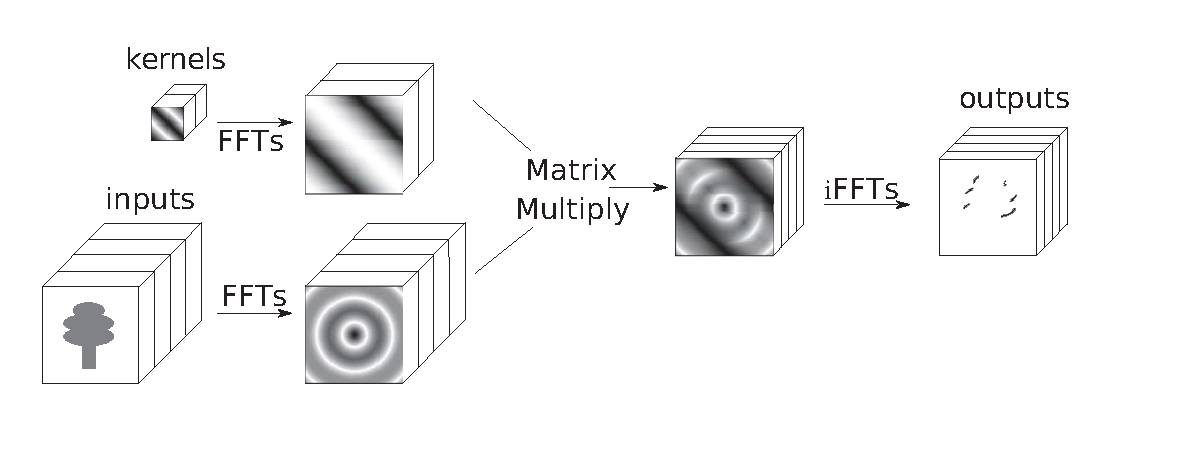
\includegraphics[width=1\columnwidth]{CNN-FFT.eps}
\caption{Block diagram showing FFT-based convolution in CNNs}
\label{CNN-FFT}
\end{center}
\end{figure}

\section{Testing}\label{section:testing}
The testing procedure will be segmented into three primary steps for each design in the project.
The first step will involve algorithmic testing in a separate C testbench similar to the usual C
simulation in Vivado HLS. This process will be conducted while experimenting with the algorithms
to improve throughput. The second step will involve using test benches within the Caffe environment
to ensure that the HLS kernels are properly integrated with the Caffe source code. Finally, the
hardware versions of the HLS kernels will be tested within the framework using the Alexnet network
against a subset of the Imagenet validation set to ensure functional correctness and accuracy
within the full system.

\section{Risk}\label{section:risk}

One primary risk for the project is that ramp up time for the toolset could be longer than
anticipated, which could result in delays with respect to finishing the design of each kernel.

\begin{itemize}
\item Identify risks attributed to your design which may cause your project to fail.
\item Provide a contingency plan, develop milestones accordingly -- see Milestones section, for example, plan a catch up week where you are not planning any deliverables.
\item Strengths and weaknesses of your team.
\end{itemize}


\section{Milestones}\label{section:milestones}
\begin{itemize}
    \item The first week will involve a ramp-up exercise to familiarize Muhammad and John with the SDAccel tools through a simple HLS kernel (e.g. "Hello World").
    \item Also in the first week, Roberto will implement a reprogram layer inside of Caffe to allow for decouple reprogramming between groups of layers.
    \item In the second week, each of us will create our C implementations of the algorithms that we are each targeting for each of the convolution layers.
    \item In the following two weeks each of us will focus on trying to improve throughput of our respective designs under the different layer constraints of AlexNet.
    \item Afterward, we will analyze the results of the respective designs, and decide which architecture will be suitable for the respective layers. Then we will begin system integration with Caffe.
    \item In the last week we will conduct additional tests of the system with images from the ImageNet validation database.
\end{itemize}


\bibliographystyle{IEEEtran}
\bibliography{references}

\end{document}
